% Chapter Template

\chapter{Analysis of Fibonacci} % Main chapter title

\label{ChapterX} % Change X to a consecutive number; for referencing this chapter elsewhere, use \ref{ChapterX}


%----------------------------------------------------------------------------------------
%	SECTION 2
%----------------------------------------------------------------------------------------

%\section{Starting With A Theorem Of Infiniteness}

%This section assumes that both P=NP and P!=NP and the following sections will %provide reasoning and examples.

%\section{Mapping Out Representations}

%This section contains my opinions of what mathematics is.

\section{Euler's Constant}

From the the reinterpretation of the theory, Euler's constant is an example of P = NP because of it's use of calculus.

$\\ $

To show that it is also in the problem set of P $\neq$ NP, start by using the picking function going into infinity.

$\\ $

$e = pf(x) = \theta(language\ of\ pf(x))$

\begin{figure}[H]
  \centering
  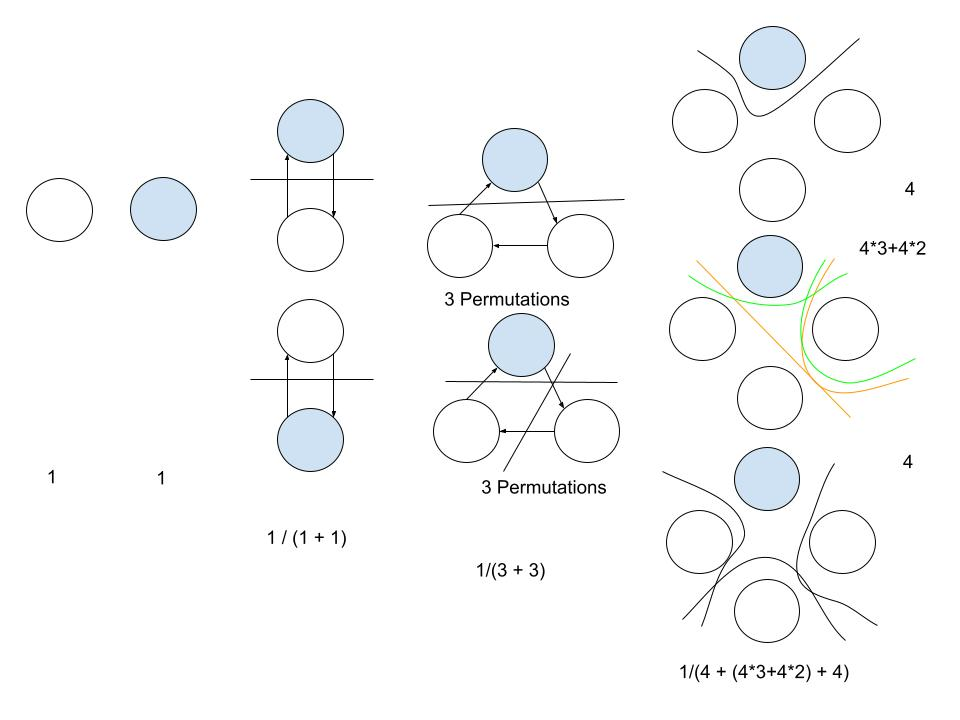
\includegraphics[width=\linewidth]{0201Eulers.jpg}
  \caption{Decider that represents the monomial, $x^3$.}
  \label{fig:0201Eulers}
\end{figure}

$\\ $

$\textit{Example}.$

$\left\{ x = x^2/x = x^3/x^2 = x^4/x^3 = x^5/x^4 = \cdots = x^n/x^{n-1} \right\}$

$e = 1 + 1 + 1/(1+1) + 1/(3+3) + 1/(4+(4*3+4*2)+4) + ...$

\section{Example of a Decider}

The following is an example of code that roughly sketches a generalized monomial decider, Decider<$2x^2$>. It tests to see if y is in the monomial m(x) = $2x^2$. Although approximation and binary search algorithms work, using this method allows for simplicity of technique in representing a decider visually and gives the reader hands-on potential if they want to experiment on the subject further.

$\\ $

% Turn into pseudocode eventually.

\begin{lstlisting}
bool generalizedDecider(int y)
{
    if (y == 0)
    {
        return true;
    }
    var s = y;
    while (s >= 0)
    {
        for (int i = 0; i < 2; i++)
        {
            for (int j = 0; j < 4; j++)
            {
                if (s == 0 && (j == 0 || j == 2) && i == 0)
                {
                    return true;
                }
                else if (s < 0)
                {
                    return false;
                }
                s -= 1;
            }
        }
    }
    return true;
}
\end{lstlisting}

$\\ $

The above code can be represented visually as follow:

\begin{figure}[H]
  \centering
  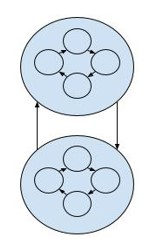
\includegraphics[scale=0.5]{0202Generalized.jpg}
  \caption{Decider that represents the monomial, $x^3$.}
  \label{fig:0202Generalized}
\end{figure}

\section{Analysis of the Decider $2x^2$}

Using the generalizedDecider function above for the Decider<$2x^2$> where a sketch of the initial algorithm is created, collecting data to find insight to make an ideal generate function: 


$\\ $

\begin{figure}[H]
  \centering
  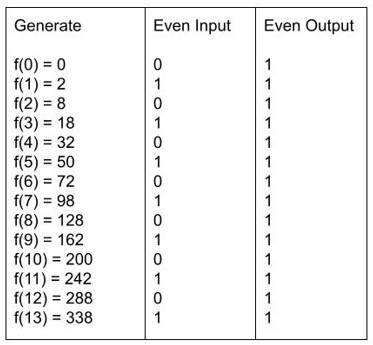
\includegraphics[width=\linewidth]{0202Generate.jpg}
  \caption{Generate function, $2x^2$.}
  \label{fig:0202Generate}
\end{figure}

$\\ $

$\textbf{Generate}$ is f(x) = $2x^2$ = y on the first line and the number of negatives is on the second. There are two finishing and all the even parity outputs end in one state and all the odd parity outputs end on the other. $\textbf{Even Input}$ is the boolean parity of the input being even. $\textbf{Even Output}$ is the boolean parity of the output being odd. 

Here, it can be seen that there is repeating pattern of even and odd values of the following:

$\\ $

$\left[ {\begin{array}{cc}
    1 & 1 \\
    0 & 1 \\
  \end{array} } \right]$

$\\ $

From this array, two finishing states are described. When the input and output are both even and one where the input is odd and the output is even. Every time the head of the tape passes a finishing state, the count of the variable, $\textbf{visit }$is increased by one. Counting the number of visits two the finishing states, it can be seen that for every pair, (start,end), there is a difference of three for $Decider<2x^2>$. The following is a table of the results:

\begin{figure}[H]
  \centering
  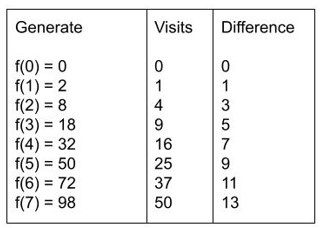
\includegraphics[width=\linewidth]{0203Visits.jpg}
  \caption{Analysis of visits to finishing states in, $2Decider<2x^2>$.}
  \label{fig:0203Visits}
\end{figure}

From analysis, the number of times the tape head visits a finishing state is the difference of the previous input plus two. The difference increases by two every time it passes a finishing state. It doesn't pass when the number of visits is even, so it can be deduced that the difference is increased by two every time it passes the odd finishing state. This result allows us to write a program to decide if y is in $2x^2$.

$\\ $
% convert to pseudocode 

\begin{lstlisting}
bool MonomialDecider2xx(int y)
{
    var totalVisits = 0;
    var currentVisits = 0;
    var diff = 1;
    var s = 0;

    while (s <= y)
    {
        for (int i = 0; i < 2; i++)
        {
            for (int j = 0; j < 2; j++)
            {
                for (int k = 0; k < 2; k++)
                {
                    if ((i == 0) && (j == 0 || j == 1) && (k == 0))
                    {
                        if (currentVisits == totalVisits)
                        {
                            if (s == y)
                            {
                                Console.WriteLine(new String("Deciding on: " + s + " - totalVisits: " + totalVisits));
                                return true;
                            }
                            else if (s > y)
                            {
                                return false;
                            }

                            totalVisits += diff;

                            // If the tape head is on the odd finishing 
                            // state increase the diff variable by 2
                            // Do this to represent x^2 in 2x^2
                            if (i == 0 && j == 1 && k == 0)
                            {
                                diff += 2;
                            }
                        }

                        currentVisits++;
                    }
                    s++;
                }
            }
        }
    }

    return false;
}
\end{lstlisting}

\section{Representing Monomial Deciders As Code}

With the data above, the requirements on constructing a decider is as follows.

Given the function:

$\\ $

$f(x)\ =\ 2x^2 = \left\{ 0,2,8,18,\cdots \right\}$

$\\ $

The output of f(x) is of the following.

x is even at 0,8,32,72

x is odd at 2,18,50

$\\ $

There are four variables constructed:

Current passes records the number of times path traveled passes a finishing state.

Total number of times traveled on a finishing state needed to reach a valid decision.

Diff is the current number of diff to increment total hits by.

IsEven is if this resets back to even, increment Diff by two.

$\\ $

The following is code generated from our more formal representation of the solution.

\begin{lstlisting}
// After getting some log results, we can construct a decider
bool MonomialDecider(int y)
{
    var isEven = 0;
    var s = 0;

    while (s <= y)
    {
        for (int i = 0; i < 2; i++)
        {
            for (int j = 0; j < 2; j++)
            {
                for (int k = 0; k < 2; k++)
                {
                    if ((i == 0)&&(j == 0 || j == 1)&&(k == 0))
                    {
                        if (hits == total)
                        {
                            if (s == y)
                            {
                                Console.WriteLine(s + ": Hits: " + total);
                                return true;
                            }
                            else if (s > y)
                            {
                                return false;
                            }

                            total += diff;
                            isEven++;
                            if (isEven % 3 == 2)
                            {
                                isEven = 0;
                                diff += 2;
                            }
                        }

                        hits++;
                    }
                    s++;
                }
            }
        }
    }

    return false;
}
\end{lstlisting}

\section{Negative Numbers}

Representing negative numbers can be thought of discretely. Below is a representaation of negative numbers.

$\\ $

Cancellation

$\\ $

Addition

$\\ $

Start and Finish: $2x$

$\\ $

Start and Finish: $x^2$

$\\ $

Ignoring the rules for commutativity and association for now.

\section{Pi}

Representing the constant pi, $\pi$, in the language of polynomials using the Leibniz formula $\pi/4 = 1 - 1/2 + 1/5 -1/7 + 1/9 + \cdots$

\section{Fibonacci}

Given the fibonacci sequence, ${1,1,2,3,5,8,13,21,\cdots}$, representing this sequence as a monomial generator in the language of polynomials can be shown below.

$\\ $

From the circles above, we see that f(1) = 1 and f(2) = 2. If we add f(1) and f(2) together we get f(3) = 3 and so on and so forth.

$\\ $

Notice that on odd inputs, Ex, there aren't any circles in the circles/states but in even inputs on X, there are two states. On outputs, Ey, it is odd twice then even once.

\begin{lstlisting}
int fibonacci(int n)
{
    if (n == 0)
    {
        return 0;
    }

    int y = 1;
    int y1 = 1;
    int y2 = 0;

    for(int i = 1; i < n; i++)
    {
        y = y1 + y2;
        y2 = y1;
        y1 = y;
    }

    return y;
}
\end{lstlisting}

\section{Analysis Of Parity In Fibonacci}

On analyzing the parity of Ex and Ey of the fibonacci sequence, we that there are two patterns.

$\\ $

$\begin{array}{ccc}
E_1 & E_2 & E_3\\
0 & 1 & 0\\
1 & 0 & 1\\
0 & 1 & 1\\
\end{array}$

$\\ $

$Det(E_1,E_2,E_3) = -1$ 

$Det(E_2,E_1,E_3) = 1$

$\\ $

$-1 + 1 -1 = -1$

$1 - 1 + 1 = 1$

\section{Redrawing the Fibonacci Sequence}

From our analysis, it can be seen that there are three states that are a minimum to create a fibonacci sequence. Minimization gives us a monomial generator, ${S_x,S_y,S_z}$. Set the three states to a desired configuration and it will generate the fibonacci sequence. It can shown that it requires three states minimum to generate the fibonacci sequence.

$\\ $

Generator

$S_x = S_y + S_z$

$S_y = S_z + S_x$

$S_z = S_x + S_y$

Using the above, dynamic programming can be modeled as a set of generator functions.

\begin{lstlisting}
int fibonacciGenerator(int n)
{
    int stateX = 0;
    int stateY = 1;
    int stateZ = 1;
    int cycles = 0;

    while (cycles <= n)
    {
        cycles++;

        if (cycles > n)
        {
            return stateX;
        }

        stateX = stateY + stateZ;
        Console.WriteLine("stateX: " + stateX + "\tstateY: " + stateY + "\tstateZ: " + stateY);
        
        cycles++;

        if (cycles > n)
        {
            return stateY;
        }

        stateY = stateX + stateZ;
        Console.WriteLine("stateX: " + stateX + "\tstateY: " + stateY + "\tstateZ: " + stateY);

        cycles++;

        if (cycles > n)
        {
            return stateZ;
        }

        stateZ = stateX + stateY;
        Console.WriteLine("stateX: " + stateX + "\tstateY: " + stateY + "\tstateZ: " + stateY);
    }

    return stateX;
}
\end{lstlisting}

\section{The Fibonacci Decider}

Given the two monomial deciders we found using the determinant, we know that we must have six numbers in the sequence to decide if they form a Fibonacci sequence. In order to create this decider, we use an addition operator to merge them together because they cancel each other out. All deciders in each set must be true in order for the sequence to be a valid Fibonacci sequence.

\section{The Fibonacci Picking Function}

Now, let's apply the picking function, pf, to the fibonacci decider and show the probability, $P_r$, of finding a sequence. $pf({xyz}_1 + {xyz}_2) = Pr({xyz}_1)*Pr({xyz}_2) \leq 1/n^{k}$

Each decider has 3 representations giving $3^2 = 9$ total for each set. We pick one decider in each set to get the probability.

There are 6 deciders with 6 permutations giving $6^2 = 36$ permutations.

This shows a concrete example of the picking function which is a type of one way function.
